\subsection{Soron belüli keretek}

%58
\begin{frame}
  Egy HTML oldal megjelenítése egy másik oldalban: \texttt{<iframe>} elemmel
  \vfill
  Attribútumok:
  \begin{description}[m]
    \item[\texttt{src}] (source) \hfill \\ A keretbe betöltendő dokumentum URL-je
    \item[\texttt{width}] \hfill \\ Keret szélessége képpontban
    \item[\texttt{height}] \hfill \\ A keret magassága képpontban
  \end{description}
\end{frame}

%59
\begin{frame}
  További attribútumok:
  \begin{description}[m]
    \item[\texttt{name}] \hfill \\ Ez azonosítja a keretet, amibe pl. új tartalom tölthető egy \texttt{<a>} elemmel, ha annak \texttt{target} attribútuma a \texttt{name} értékét tartalmazza
    \item[\texttt{srcdoc}] \hfill \\ Megjelenítendő dokumentum HTML kódja (magasabb prioritású, mint \texttt{src}, ha támogatott)
    \item[\texttt{sandbox}] \hfill \\ Megjelenítési környezet korlátozásainak feloldása (\texttt{allow-forms}, \texttt{allow-pointer-lock}, \texttt{allow-popups}, \texttt{allow-same-origin}, \texttt{allow-scripts}, \texttt{allow-top-navigation}) \hiv{\href{https://www.html5rocks.com/en/tutorials/security/sandboxed-iframes/}{részletek}}
  \end{description}
\end{frame}

%60
\begin{frame}
  Megjegyzések
  \begin{itemize}
    \item Az \texttt{srcdoc}-ot csak az \hiv{\href{https://caniuse.com/\#search=iframe\%20srcdoc}{újabb}} böngészők támogatják
    \item A webszerverek az \hiv{\href{https://developer.mozilla.org/hu/docs/Web/HTTP/Headers/X-Frame-Options}{X-Frame-Options}} HTTP válasz fejléccel kérhetik az ezt támogató böngészőktől, hogy ne engedjék a lapot \texttt{<iframe>}-be tölteni.
    \item \texttt{src}+\texttt{sandbox} biztonságos korszerű böngészőkben, de \kiemel{nem biztonságos a \texttt{sandbox}-ot nem támogatókban!}
    \item \texttt{srcdoc}+\texttt{sandbox} biztonságos korszerű böngészőkben, és nem működik (=biztonságos) az elavultakban
  \end{itemize}
\end{frame}

%61
\begin{frame}
  \begin{columns}[c]
    \column{0.6\textwidth}
      \begin{exampleblock}{\textattachfile{iframe.html}{iframe.html}}
        \footnotesize
        \lstinputlisting[style=HTML,linerange={8-14},numbers=left,firstnumber=8]{iframe.html}
      \end{exampleblock}
    \column{0.35\textwidth}
      \centering 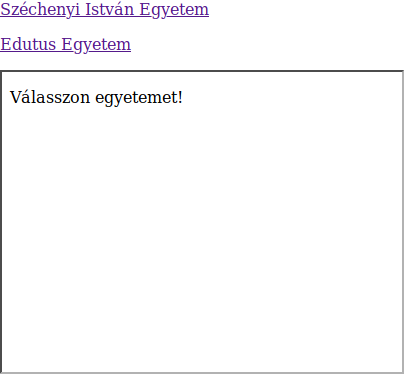
\includegraphics[width=\textwidth]{iframe.png}
  \end{columns}
\end{frame}
